%  A simple AAU report template.
%  2015-05-08 v. 1.2.0
%  Copyright 2010-2015 by Jesper Kjær Nielsen <jkn@es.aau.dk>
%
%  This is free software: you can redistribute it and/or modify
%  it under the terms of the GNU General Public License as published by
%  the Free Software Foundation, either version 3 of the License, or
%  (at your option) any later version.
%
%  This is distributed in the hope that it will be useful,
%  but WITHOUT ANY WARRANTY; without even the implied warranty of
%  MERCHANTABILITY or FITNESS FOR A PARTICULAR PURPOSE.  See the
%  GNU General Public License for more details.
%
%  You can find the GNU General Public License at <http://www.gnu.org/licenses/>.
%
\documentclass[11pt,a4paper,openright]{report}
%%%%%%%%%%%%%%%%%%%%%%%%%%%%%%%%%%%%%%%%%%%%%%%%
% Language, Encoding and Fonts
% http://en.wikibooks.org/wiki/LaTeX/Internationalization
%%%%%%%%%%%%%%%%%%%%%%%%%%%%%%%%%%%%%%%%%%%%%%%%
% Select encoding of your inputs. Depends on
% your operating system and its default input
% encoding. Typically, you should use
%   Linux  : utf8 (most modern Linux distributions)
%            latin1 
%   Windows: ansinew
%            latin1 (works in most cases)
%   Mac    : applemac
% Notice that you can manually change the input
% encoding of your files by selecting "save as"
% an select the desired input encoding. 
\usepackage[utf8]{inputenc}
% Make latex understand and use the typographic
% rules of the language used in the document.
\usepackage[english, danish]{babel}
% Use the palatino font
\usepackage[sc]{mathpazo}
\linespread{1.05}         % Palatino needs more leading (space between lines)
% Choose the font encoding
\usepackage[T1]{fontenc}
%%%%%%%%%%%%%%%%%%%%%%%%%%%%%%%%%%%%%%%%%%%%%%%%
% Graphics and Tables
% http://en.wikibooks.org/wiki/LaTeX/Importing_Graphics
% http://en.wikibooks.org/wiki/LaTeX/Tables
% http://en.wikibooks.org/wiki/LaTeX/Colors
%%%%%%%%%%%%%%%%%%%%%%%%%%%%%%%%%%%%%%%%%%%%%%%%
% load a colour package
\usepackage[dvipsnames]{xcolor}
\definecolor{aaublue}{RGB}{33,26,82}% dark blue
% The standard graphics inclusion package
\usepackage{graphicx}
% Set up how figure and table captions are displayed
\usepackage{float}
\usepackage{caption}
\captionsetup{%
  font=footnotesize,% set font size to footnotesize
  labelfont=bf % bold label (e.g., Figure 3.2) font
}
% Make the standard latex tables look so much better
\usepackage{array,booktabs}
% Enable the use of frames around, e.g., theorems
% The framed package is used in the example environment
\usepackage{framed}
\usepackage{wrapfig}
\usepackage{multirow}

%%%%%%%%%%%%%%%%%%%%%%%%%%%%%%%%%%%%%%%%%%%%%%%%
% Mathematics
% http://en.wikibooks.org/wiki/LaTeX/Mathematics
%%%%%%%%%%%%%%%%%%%%%%%%%%%%%%%%%%%%%%%%%%%%%%%%
% Defines new environments such as equation,
% align and split 
\usepackage{amsmath}
% Adds new math symbols
\usepackage{amssymb}
% Use theorems in your document
% The ntheorem package is also used for the example environment
% When using thmmarks, amsmath must be an option as well. Otherwise \eqref doesn't work anymore.
\usepackage[framed,amsmath,thmmarks]{ntheorem}

%%%%%%%%%%%%%%%%%%%%%%%%%%%%%%%%%%%%%%%%%%%%%%%%
% Page Layout
% http://en.wikibooks.org/wiki/LaTeX/Page_Layout
%%%%%%%%%%%%%%%%%%%%%%%%%%%%%%%%%%%%%%%%%%%%%%%%
% Change margins, papersize, etc of the document
\usepackage[
  inner=30mm,% left margin on an odd page
  outer=30mm,% right margin on an odd page
  ]{geometry}
% Modify how \chapter, \section, etc. look
% The titlesec package is very configureable
\usepackage{titlesec}
\titleformat{\chapter}[display]{\normalfont\huge\bfseries}{\ }{20pt}{\Huge}
\titleformat*{\section}{\normalfont\Large\bfseries}
\titleformat*{\subsection}{\normalfont\large\bfseries}
\titleformat*{\subsubsection}{\normalfont\normalsize\bfseries}
\titleformat*{\paragraph}{\normalfont\normalsize\bfseries}
\titleformat*{\subparagraph}{\normalfont\normalsize\bfseries}

% Clear empty pages between chapters
\let\origdoublepage\cleardoublepage
\newcommand{\clearemptydoublepage}{%
  \clearpage
  {\pagestyle{empty}\origdoublepage}%
}
\let\cleardoublepage\clearemptydoublepage

% Change the headers and footers
\usepackage{fancyhdr}
\pagestyle{fancy}
\fancyhf{} %delete everything
\renewcommand{\headrulewidth}{0pt} %remove the horizontal line in the header
\fancyhead[R]{\small\nouppercase\leftmark} %even page - chapter title
\fancyhead[LO]{\small\nouppercase\rightmark} %uneven page - section title
\fancyhead[RO]{\thepage} %page number on all pages
\setlength{\headheight}{13.59999pt}
% Do not stretch the content of a page. Instead,
% insert white space at the bottom of the page
\raggedbottom
% Enable arithmetics with length. Useful when
% typesetting the layout.
\usepackage{calc}

%Paragraph spacing
\setlength{\parindent}{0em}
\setlength{\parskip}{1em}

%%%%%%%%%%%%%%%%%%%%%%%%%%%%%%%%%%%%%%%%%%%%%%%%
% Misc
%%%%%%%%%%%%%%%%%%%%%%%%%%%%%%%%%%%%%%%%%%%%%%%%
% Add bibliography and index to the table of
% contents
\usepackage[nottoc]{tocbibind}
% Add the command \pageref{LastPage} which refers to the
% page number of the last page
\usepackage{lastpage}
% Add todo notes in the margin of the document
\usepackage[
%  disable, %turn off todonotes
  colorinlistoftodos, %enable a coloured square in the list of todos
  textwidth=\marginparwidth, %set the width of the todonotes
  textsize=scriptsize, %size of the text in the todonotes
  ]{todonotes}
% include pdf files
\usepackage[final]{pdfpages}
% code
\usepackage{color}
\usepackage{listings}
\usepackage{tcolorbox}
\usepackage{subfig}
% coding colors defined %
\definecolor{codegreen}{rgb}{0,0.6,0}
\definecolor{codegray}{rgb}{0.5,0.5,0.5}
\definecolor{codepurple}{rgb}{0.58,0,0.82}
\definecolor{backcolour}{rgb}{0.95,0.95,0.92}

 
\lstdefinestyle{JavaStyle}{
    backgroundcolor=\color{backcolour},   
    commentstyle=\color{codegreen},
    keywordstyle=\color{magenta},
    numberstyle=\tiny\color{codegray},
    stringstyle=\color{codepurple},
    basicstyle=\footnotesize,
    breakatwhitespace=false,         
    breaklines=true,                 
    captionpos=b,
    frame=single,
    keepspaces=true,                 
    numbers=left,                    
    numbersep=5pt,                  
    showspaces=false,                
    showstringspaces=false,
    showtabs=false,
    language=Java,
    tabsize=4,
    extendedchars=true,
    literate={æ}{{\ae}}1 {Æ}{{\AE}}1 {ø}{{\o}}1 {Ø}{{\O}}1 {å}{{\r a}}1 {Å}{{\r A}}1,
}

\lstdefinelanguage{JavaScript}{
%alsoletter=æøå,
keywords={metode, liste, Dec, udskriv, hvis, tilføj, returner, hent, længde, somHeltal, Hel, imens, indsæt, ordbog, tekst, størrelse, nøgler},
keywordstyle=\color{blue}\bfseries,
ndkeywords={start},
ndkeywordstyle=\color{darkgray}\bfseries,
identifierstyle=\color{black},
sensitive=false,
comment=[l]{//},
morecomment=[s]{/*}{*/},
commentstyle=\color{purple}\ttfamily,
stringstyle=\color{red}\ttfamily,
morestring=[b]',
morestring=[b]"
}

\lstdefinestyle{JavaScriptStyle}{
    backgroundcolor=\color{backcolour},   
    commentstyle=\color{codegreen},
    keywordstyle=\color{magenta},
    numberstyle=\tiny\color{codegray},
    stringstyle=\color{codepurple},
    basicstyle=\footnotesize,
    breakatwhitespace=false,         
    breaklines=true,                 
    captionpos=b,
    frame=single,
    keepspaces=true,                 
    numbers=left,                    
    numbersep=5pt,                  
    showspaces=false,                
    showstringspaces=false,
    showtabs=false,
    language=javascript,
    tabsize=4,
    extendedchars=true,
    literate={æ}{{\ae}}1 {Æ}{{\AE}}1 {ø}{{\o}}1 {Ø}{{\O}}1 {å}{{\r a}}1 {Å}{{\r A}}1,
}
\lstset{style=JavaStyle}
\renewcommand{\lstlistingname}{Code}% Listing -> Code
\renewcommand{\lstlistlistingname}{List of \lstlistingname}% List of Listings -> List of Code
%%%%%%%%%%%%%%%%%%%%%%%%%%%%%%%%%%%%%%%%%%%%%%%%
% Hyperlinks
% http://en.wikibooks.org/wiki/LaTeX/Hyperlinks
%%%%%%%%%%%%%%%%%%%%%%%%%%%%%%%%%%%%%%%%%%%%%%%%
% Enable hyperlinks and insert info into the pdf
% file. Hypperref should be loaded as one of the 
% last packages

\usepackage{multirow}
\usepackage{csquotes}
\usepackage{chngpage}
\usepackage{pdflscape}
\usepackage{longtable}
\usepackage{makecell}

\usepackage[nobreak]{mdframed}

\numberwithin{equation}{chapter}

\usepackage{csvsimple}

\usepackage{tikz}
\usetikzlibrary{matrix}

\titlespacing*{\chapter}{0pt}{0pt}{40pt}
\usepackage{ulem}

\mdfdefinestyle{drikstyle}{%
linecolor=CornflowerBlue,linewidth=2pt,%
frametitlerule=true,%
frametitlebackgroundcolor=CornflowerBlue!20,
innertopmargin=\topskip,
}
\mdtheorem[style=drikstyle]{drik}{Drik}

\mdfdefinestyle{særligstyle}{%
linecolor=SpringGreen,linewidth=2pt,%
frametitlerule=true,%
frametitlebackgroundcolor=SpringGreen!20,
innertopmargin=\topskip,
}
\mdtheorem[style=særligstyle]{særlig}{Særlig}

\mdfdefinestyle{giftstyle}{%
linecolor=Bittersweet,linewidth=2pt,%
frametitlerule=true,%
frametitlebackgroundcolor=Bittersweet!20,
innertopmargin=\topskip,
}
\mdtheorem[style=giftstyle]{gift}{Gift}

\mdfdefinestyle{artefaktstyle}{%
linecolor=BlueGreen,linewidth=2pt,%
frametitlerule=true,%
frametitlebackgroundcolor=BlueGreen!20,
innertopmargin=\topskip,
}
\mdtheorem[style=artefaktstyle]{artefakt}{Artefakt}

\mdfdefinestyle{runerustningstyle}{%
linecolor=Emerald,linewidth=2pt,%
frametitlerule=true,%
frametitlebackgroundcolor=Emerald!20,
innertopmargin=\topskip,
}
\mdtheorem[style=runerustningstyle]{runerustning}{Runerustning}

\mdfdefinestyle{runevåbenstyle}{%
linecolor=RoyalBlue,linewidth=2pt,%
frametitlerule=true,%
frametitlebackgroundcolor=RoyalBlue!20,
innertopmargin=\topskip,
}
\mdtheorem[style=runevåbenstyle]{runevåben}{Runevåben}

\mdfdefinestyle{runeskjoldstyle}{%
linecolor=RoyalPurple,linewidth=2pt,%
frametitlerule=true,%
frametitlebackgroundcolor=RoyalPurple!20,
innertopmargin=\topskip,
}
\mdtheorem[style=runeskjoldstyle]{runeskjold}{Runeskjold}

\usepackage{tablefootnote}

\mdfdefinestyle{Meditationstyle}{%
linecolor=Emerald,linewidth=2pt,%
frametitlerule=true,%
frametitlebackgroundcolor=Emerald!20,
innertopmargin=\topskip,
}
\mdtheorem[style=Meditationstyle]{meditation}{Meditation}

\mdfdefinestyle{Orleksarvstyle}{%
linecolor=RedOrange,linewidth=2pt,%
frametitlerule=true,%
frametitlebackgroundcolor=RedOrange!20,
innertopmargin=\topskip,
}
\mdtheorem[style=Orleksarvstyle]{orleks arv}{Orleks arv}
\mdtheorem[style=Orleksarvstyle]{dHævn}{Dæmonisk hævn}

\mdfdefinestyle{Ritualstyle}{%
linecolor=Magenta,linewidth=2pt,%
frametitlerule=true,%
frametitlebackgroundcolor=Magenta!20,
innertopmargin=\topskip,
}
\mdtheorem[style=Ritualstyle]{ritual}{Ritual}

\mdfdefinestyle{Åndensgavestyle}{%
linecolor=RoyalBlue,linewidth=2pt,%
frametitlerule=true,%
frametitlebackgroundcolor=RoyalBlue!20,
innertopmargin=\topskip,
}
\mdtheorem[style=Åndensgavestyle]{åndens gave}{Åndernes gave}

\mdtheorem[style=Meditationstyle]{nBeskyt}{Naturens Beskyttelse}

\mdfdefinestyle{naturstyle}{%
linecolor=Goldenrod,linewidth=2pt,%
frametitlerule=true,%
frametitlebackgroundcolor=Goldenrod!20,
innertopmargin=\topskip,
}
\mdtheorem[style=naturstyle]{nly}{Naturens Ly}

\mdtheorem[style=drikstyle]{nvit}{Naturens Vitalitet}

\mdtheorem[style=særligstyle]{mkær}{Moder Naturs Kærlighed}

\mdtheorem[style=giftstyle]{nhævn}{Naturens hævn}

\mdtheorem[style=Åndensgavestyle]{nkaos}{Naturens Kaos}

\mdtheorem[style=runeskjoldstyle]{nbesk}{Naturens Beskyttelse}

\mdfdefinestyle{primærstyle}{%
linecolor=Plum,linewidth=2pt,%
frametitlerule=true,%
frametitlebackgroundcolor=Plum!20,
innertopmargin=\topskip,
}
\mdtheorem[style=primærstyle]{primærMagi}{Primær Magi}

\mdfdefinestyle{Lærdstyle}{%
linecolor=SkyBlue,linewidth=2pt,%
frametitlerule=true,%
frametitlebackgroundcolor=SkyBlue!20,
innertopmargin=\topskip,
}
\mdtheorem[style=Lærdstyle]{lærdMagi}{Den Lærdes Vej}

\mdfdefinestyle{ArkBanestyle}{%
linecolor=SeaGreen,linewidth=2pt,%
frametitlerule=true,%
frametitlebackgroundcolor=SeaGreen!20,
innertopmargin=\topskip,
}
\mdtheorem[style=ArkBanestyle]{arkBaneMagi}{Arkanaens Bane}

\mdfdefinestyle{magiMesterstyle}{%
linecolor=Orange,linewidth=2pt,%
frametitlerule=true,%
frametitlebackgroundcolor=Orange!20,
innertopmargin=\topskip,
}
\mdtheorem[style=magiMesterstyle]{mesterMagi}{Magiens Mester}

\mdfdefinestyle{sAritstyle}{%
linecolor=Melon,linewidth=2pt,%
frametitlerule=true,%
frametitlebackgroundcolor=Melon!20,
innertopmargin=\topskip,
}
\mdtheorem[style=sAritstyle]{sAritMagi}{Sfære Aritmetik}

\usepackage[T1]{fontenc} %thanks's daleif
\usepackage[utf8]{inputenc}
\usepackage[english, danish]{babel}
\newcommand{\tabitem}{~~\llap{\textbullet}~~}

\mdfdefinestyle{racestyle}{%
linecolor=PineGreen,linewidth=2pt,%
frametitlerule=true,%
frametitlebackgroundcolor=PineGreen!20,
innertopmargin=\topskip,
}
\mdtheorem[style=sAritstyle]{race}{Race Detaljer}

\mdfdefinestyle{sjælstyle}{%
linecolor=Cyan,linewidth=2pt,%
frametitlerule=true,%
frametitlebackgroundcolor=Cyan!20,
innertopmargin=\topskip,
}
\mdtheorem[style=sjælstyle]{sjæl}{Sælg din Sjæl}

\mdfdefinestyle{Korruptionstyle}{%
linecolor=PineGreen,linewidth=2pt,%
frametitlerule=true,%
frametitlebackgroundcolor=PineGreen!20,
innertopmargin=\topskip,
}
\mdtheorem[style=Korruptionstyle]{korruption}{Korruption}

\mdfdefinestyle{Faldenstyle}{%
linecolor=Tan,linewidth=2pt,%
frametitlerule=true,%
frametitlebackgroundcolor=Tan!20,
innertopmargin=\topskip,
}
\mdtheorem[style=Faldenstyle]{falden}{Falden Engel}

\mdfdefinestyle{Vandstyle}{%
linecolor=Aquamarine,linewidth=2pt,%
frametitlerule=true,%
frametitlebackgroundcolor=Aquamarine!20,
innertopmargin=\topskip,
}
\mdtheorem[style=Vandstyle]{vand}{Vand}

\mdfdefinestyle{Ildstyle}{%
linecolor=BrickRed,linewidth=2pt,%
frametitlerule=true,%
frametitlebackgroundcolor=BrickRed!20,
innertopmargin=\topskip,
}
\mdtheorem[style=Ildstyle]{ild}{Ild}

\mdfdefinestyle{Jordstyle}{%
linecolor=Sepia,linewidth=2pt,%
frametitlerule=true,%
frametitlebackgroundcolor=Sepia!20,
innertopmargin=\topskip,
}
\mdtheorem[style=Jordstyle]{jord}{Jord}

\mdfdefinestyle{Vindstyle}{%
linecolor=Gray,linewidth=2pt,%
frametitlerule=true,%
frametitlebackgroundcolor=Gray!20,
innertopmargin=\topskip,
}
\mdtheorem[style=Vindstyle]{vind}{Vind}

\mdtheorem[style=naturstyle]{passiv}{Passiv}

\mdtheorem[style=ArkBanestyle]{offensiv}{Offensiv}

\mdtheorem[style=runevåbenstyle]{defensiv}{Defensiv}

\mdtheorem[style=giftstyle]{kontrol}{Kontrol}

\mdtheorem[style=særligstyle]{zombie}{Zombie}

\mdtheorem[style=Orleksarvstyle]{nSjæl}{Sjæl}

\mdtheorem[style=Åndensgavestyle]{sygdom}{Sygdomens Mørke}

\mdtheorem[style=Ritualstyle]{død}{Død}

\mdtheorem[style=Ritualstyle]{prof}{Profession}% package inclusion and set up of the document
% see, e.g., http://en.wikibooks.org/wiki/LaTeX/Formatting#Hyphenation
% for more information on word hyphenation
\hyphenation{ex-am-ple hy-phen-a-tion short}
\hyphenation{long la-tex}% 
%  A simple AAU report template.
%  2015-05-08 v. 1.2.0
%  Copyright 2010-2015 by Jesper Kjær Nielsen <jkn@es.aau.dk>
%
%  This is free software: you can redistribute it and/or modify
%  it under the terms of the GNU General Public License as published by
%  the Free Software Foundation, either version 3 of the License, or
%  (at your option) any later version.
%
%  This is distributed in the hope that it will be useful,
%  but WITHOUT ANY WARRANTY; without even the implied warranty of
%  MERCHANTABILITY or FITNESS FOR A PARTICULAR PURPOSE.  See the
%  GNU General Public License for more details.
%
%  You can find the GNU General Public License at <http://www.gnu.org/licenses/>.
%
%
%
% see, e.g., http://en.wikibooks.org/wiki/LaTeX/Customizing_LaTeX#New_commands
% for more information on how to create macros

%%%%%%%%%%%%%%%%%%%%%%%%%%%%%%%%%%%%%%%%%%%%%%%%
% Macros for the titlepage
%%%%%%%%%%%%%%%%%%%%%%%%%%%%%%%%%%%%%%%%%%%%%%%%
%Creates the aau titlepage
\newcommand{\aautitlepage}[3]{%
  {
    %set up various length
    \ifx\titlepageleftcolumnwidth\undefined
      \newlength{\titlepageleftcolumnwidth}
      \newlength{\titlepagerightcolumnwidth}
    \fi
    \setlength{\titlepageleftcolumnwidth}{0.5\textwidth-\tabcolsep}
    \setlength{\titlepagerightcolumnwidth}{\textwidth-2\tabcolsep-\titlepageleftcolumnwidth}
    %create title page
    \thispagestyle{empty}
    \noindent%
    \begin{tabular}{@{}ll@{}}
      \parbox{\titlepageleftcolumnwidth}{
        \iflanguage{danish}{%
          \includegraphics[width=\titlepageleftcolumnwidth]{figures/aau_logo_da}
        }{%
          \includegraphics[width=\titlepageleftcolumnwidth]{figures/aau_logo_en}
        }
      } &
      \parbox{\titlepagerightcolumnwidth}{\raggedleft\sf\small
        #2
      }\bigskip\\
       #1 &
      \parbox[t]{\titlepagerightcolumnwidth}{%
      \textbf{Abstract:}\bigskip\par
        \fbox{\parbox{\titlepagerightcolumnwidth-2\fboxsep-2\fboxrule}{%
          #3
        }}
      }\\
    \end{tabular}
    \vfill
    \iflanguage{danish}{%
      \noindent{\footnotesize\emph{Rapportens indhold er frit tilgængeligt, men offentliggørelse (med kildeangivelse) må kun ske efter aftale med forfatterne.}}
    }{%
      \noindent{\footnotesize\emph{The content of this report is freely available, but publication (with reference) may only be pursued due to agreement with the author.}}
    }
    \clearpage
  }
}

%Create english project info
\newcommand{\englishprojectinfo}[8]{%
  \parbox[t]{\titlepageleftcolumnwidth}{
    \textbf{Title:}\\ #1\bigskip\par
    \textbf{Theme:}\\ #2\bigskip\par
    \textbf{Project Period:}\\ #3\bigskip\par
    \textbf{Project Group:}\\ #4\bigskip\par
    \textbf{Participant(s):}\\ #5\bigskip\par
    \textbf{Supervisor(s):}\\ #6\bigskip\par
    \textbf{Page Numbers:} \pageref{LastPage}\bigskip\par
    \textbf{Date of Completion:}\\ #8
  }
}

%Create danish project info
\newcommand{\danishprojectinfo}[8]{%
  \parbox[t]{\titlepageleftcolumnwidth}{
    \textbf{Titel:}\\ #1\bigskip\par
    \textbf{Tema:}\\ #2\bigskip\par
    \textbf{Projektperiode:}\\ #3\bigskip\par
    \textbf{Projektgruppe:}\\ #4\bigskip\par
    \textbf{Deltager(e):}\\ #5\bigskip\par
    \textbf{Vejleder(e):}\\ #6\bigskip\par
    \textbf{Oplagstal:} #7\bigskip\par
    \textbf{Sidetal:} \pageref{LastPage}\bigskip\par
    \textbf{Afleveringsdato:}\\ #8
  }
}

%%%%%%%%%%%%%%%%%%%%%%%%%%%%%%%%%%%%%%%%%%%%%%%%
% An example environment
%%%%%%%%%%%%%%%%%%%%%%%%%%%%%%%%%%%%%%%%%%%%%%%%
\theoremheaderfont{\normalfont\bfseries}
\theorembodyfont{\normalfont}
\theoremstyle{break}
\def\theoremframecommand{{\color{gray!50}\vrule width 5pt \hspace{5pt}}}
\newshadedtheorem{exa}{Example}[chapter]
\newenvironment{example}[1]{%
		\begin{exa}[#1]
}{%
		\end{exa}
}% my new macros
\usepackage{xcolor,colortbl}
\definecolor{Gray}{gray}{0.85}
\newcolumntype{a}{>{\columncolor{Gray}}c}
\newcolumntype{b}{>{\columncolor{white}}c}
\definecolor{maroon}{cmyk}{0,0.87,0.68,0.32}
\definecolor{bleudefrance}{rgb}{0.19, 0.55, 0.91}
\definecolor{cerulean}{rgb}{0.0, 0.48, 0.65}
\usepackage{hyperref}
\hypersetup{%
	%pdfpagelabels=true,%
	plainpages=false,%
	pdfauthor={Akastin},%
	pdftitle={Det Generelle Regelsæt},%
	pdfsubject={Regler},%
	bookmarksnumbered=true,%
	colorlinks=true,%
	citecolor=black,%
	filecolor=blue,%
	linkcolor=black,% you should probably change this to black before printing
	urlcolor=blue,%
	pdfstartview=FitH,%
	bookmarksopen=true
}
\usepackage{stmaryrd}

\begin{document}
\begin{titlepage}
    \begin{center}
        \includegraphics[width=0.95\textwidth]{setup/Pictures/A01.C01.01_Front_Billede.png}
        
        \vspace{0.5cm}
        \LARGE
        \textit{Regelsæt for}
        
        \vspace{4.5cm}
        \Huge
        \textbf{De Generelle Regler}\\
        \vspace{4.5cm}
        \large
        \textit{Opdateret: \today}
\end{center}
\end{titlepage}

\pagestyle{plain} %enable headers and footers again
%mainmatter
\pagenumbering{arabic} %use arabic page numbering in the mainmatter
\renewcommand*\contentsname{Indholdsfortegnelse}
\tableofcontents
\chapter{Liverollespil i A’kastin}
Der findes mange former for rollespil. I A’kastin spiller vi High Fantasy. Magi, magiske væsner, guder og liv efter døden er derfor normalt her.\\
\textbf{Karakter:} Når du spiller, skal du have en karakter i form af et karakterark. Dette ark kan du selv lave via. hjemmesiden, eller du kan møde op til en spilgang og få hjælp af en arrangør ved tjek ind. Fælles er, at det skal være printet ud, eller være på din telefon, og fremvises til arrangørerne til hver spilgang.\\
Denne karakter er din rolle, ligesom i et skuespil. Forskellen på et skuespil og det vi laver i A’kastin, er at dine replikker og din skæbne ikke er bestemt på forhånd i liverollespil. Det er derfor helt op til dig, hvordan du vil udvikle din karakter.\\
\textbf{In-game og off-game:} In-game er, når du er inde i spillet, som den karakter du har lavet et karakterark til. In-game er adskilt fra off-game, for at bibeholde illusionen om, at du nu befinder dig i en anden verden. Du må derfor ikke gå off-game midt i spillet. Har du brug for en pause, er der områder, hvor du kan gå off-game.\\
\textbf{Er du ny:} Hvis du er ny til liverollespil, anbefaler vi, at du ser på fanen “For nye spillere” på hjemmesiden. Fanen ligger under “Information”.\\

\section{Arrangørerne}
I A’kastin er det Live Fantasy Arrangørgruppen, der arrangerer rollespillet, og det er dermed også dem, der bestemmer til spilgangene.\\
Følger du ikke deres anvisninger, kan det i værste fald medføre bortvisning.\\
Er du i tvivl om hvem, der er medlem af arrangørgruppen, kan du se det inde på vores hjemmeside.\\
Officiel kommunikation med arrangørerne skal foregå over mail til akastin@gmail.com.\\

\section{Opførsel i bakkerne}
Spilområdet er et fredet naturområde, som vi låner. Fordi det er fredet, er der følgende regler, som skal overholdes:
\begin{itemize}
    \item Lyngen i bakkerne er fredet. Træd ikke på det, men brug de anviste stier.
    \item Lad være med at gøre skade på naturen. Hertil hører, at du for eksempel ikke må knække grene af træer eller fælde dem.
    \item Smid ikke dit affald i naturen. Smid det i en skraldespand.
    \item Hop ikke over hegnet. Brug lågerne der findes flere steder i området.
    \item Åben ild er forbudt i bakkerne. Dette gælder også trangia sæt.
    \item A’kastin rollespilsforening befinder sig i Rebild kommune, som er en røgfri kommune. Det er derfor forbudt at ryge på spilområdet. Ønsker man at ryge skal dette gøres på parkeringspladsen.
    \item Der er dyr i bakkerne, dette er normalt får. Disse har fortrins ret, og må ikke slås på. Hvis de løber mod dig, så er det din opgave at bakke væk.
    \item Brug de anviste toiletter, og gør rent efter dig selv (sminkning og lignende).
\end{itemize}
Overholdes disse regler ikke kan det medføre bøder.

\section{Retningslinjer for A’kastins livearrangementer}
Når du deltager i vores arrangementer, giver du samtykke til, at der bliver taget billeder og videoer, som bliver lagt op på vores hjemmeside, officielle facebookside og brugt til reklame for foreningen. Arrangørerne kan ikke drages til ansvar for billeder, som er taget eller bruges af privatpersoner. Har du indvendinger, bedes du kontakte arrangørgruppen over mail på akastin@gmail.com.
\chapter*{Regler for spillet}\addcontentsline{toc}{chapter}{Regler for spillet}
\section*{Tjek ind}\addcontentsline{toc}{section}{Tjek ind}

For at kunne deltage til spilgangene, skal du tjekkes ind. Dette foregår på parkeringspladsen, før vi laver en spilbriefing. Her vil du få udleveret in-game genstande og kan stille spørgsmål til arrangørerne.\\
Samtidig med tjek ind er der også våben- og rustningstjek. Alle våben og rustninger skal checkes før spilgangene, også selvom de er blevet godkendt til tidligere scenarier. Vi anbefaler, at man anskaffer sig
våben og rustning fra officielle rollespilsbutikker, da vi har erfaring med, at våben fra Netto, Fakta osv. ikke klarer sikkerhedschecket.\\
Har du brug for at tjekke ind udenfor normalt tidsrum, bedes du kontakte en arrangør.

\section*{In-game}\addcontentsline{toc}{section}{In-game}
Når du er in-game, spiller du din rolle og befinder dig i verdenen Kalish. Din rolle er baseret på race, profession, religion og baggrundshistorie. Din rolle har egne ambitioner og mål, som denne gerne vil føre ud i livet.\\
Konceptet med in-game er, at du spiller din rolle, så det er tydeligt, at du befinder dig i en anden verden. Det vil sige, at in-game foregår udenfor din normale hverdag; mobiltelefoner, snak om familiens kæledyr og lignende, vil vi derfor ikke opleve in-game.

\section*{In-game kulisser}\addcontentsline{toc}{section}{In-game kulisser}
\textbf{Telte:} Foreningen opstiller middelaldertelte til hver spilgang. Disse telte fungere som in-game bygninger. Du er altid velkommen til at tage dit eget middelaldertelt med og sætte op.\\
\textbf{Mure:} Mure er kun gældende som mure, hvis de opfylder ét af følgende punkter:
\begin{itemize}
    \item Den er lavet af en form for stof (f.eks. stofsider i et telt)
    \item Den er lavet af en presenning.
    \item Den er en reel mur, der er lavet af eksempelvis træplader eller andet hårdt materiale
\end{itemize}

Bunker af grene der er stablet, er derfor ikke gældende som mur, og er udelukkende en forhindring, som kan gås igennem.\\
Vælger en spiller at lave en mur, skal denne, selvom den opfylder ovenstående ét af ovenstående punkter, godkendes af en arrangør.\\
\textbf{Porte og døre:} En dør er bl.a. indgangen til en bygning og en port er en passage i en mur. Disse skal være synlige, og det skal være åbenlyst, at det er en indgang.\\
Porte og døre kan være låste, hvilket skal markeres med en in-game lås. Det er ikke tilladt, at fysisk blokere en dør eller port. For at komme forbi låsen skal du bruge en af følgende metoder:
\begin{itemize}
    \item Man har nøglen til låsen.
    \item Ved brug af evner.
    \item Man kan bruge en rambuk. Det kræver minimum 5 personer med en samlet nævekamp(Nævekamp forklares længere nede.) på 20. Det tager 2 minutter at nedbryde en dør og 10 minutter for en port. Det er ikke tilladt at ramme døren og dermed ødelægge den rigtigt. Situationen skal rollespilles/markeres for både døre og porte.
\end{itemize}

\section*{In-game værdier}\addcontentsline{toc}{section}{In-game værdier}
Fjend er vores møntfod (opkaldt efter kejserfamilien Fjendebane i Nordland), og det er dem, du bruger til at betale for in-game genstande.\\
In-game genstande kan være alt fra mad til magiske artefakter. disse må hverken graves ned eller gemmes væk off-game. Hvis du bærer genstandene på dig, der ikke er beskyttet af en lås, skal disse ting afleveres, hvis du bliver gennemsøgt, når du er død. Her er det vigtigt at huske, at det ikke er tilladt at tage de sidste 3 Fjend på en person. Stjæler du fra en kiste, må du tage alle genstande i kisten med dig.\\
Bærer du in-game værdier, skal du være sikker på ikke at tabe dem rundt om i skoven.

\section*{Off-game}\addcontentsline{toc}{section}{Off-game}
Når du er off-game spiller du ikke længere din rolle, men er dig selv. Det vil sige, at du ikke må snakke med spillere, der er in-game eller på anden måde interagere med spillet. Som off-game kan du bruge din telefon mm., men det skal foregå udenfor spilområdet.\\
Når du er off-game, skal du lægge en hånd eller begge dine hænder på hovedet. Det er ikke tilladt at gå off-game midt i spillet. Herunder hører, at du ikke må “forsvinde” off-game for at undgå en kamp/konflikt. Du må heller ikke stoppe spillet, for at diskutere regler. Er du i tvivl om noget, kan du spørge en arrangør.

\section*{Kommunikation}\addcontentsline{toc}{section}{Kommunikation}
Vi forventer, at der holdes en god tone mellem alle personer, der deltager i A’kastin såvel i spillet som udenfor spillet. Du må selvfølgelig gerne rollespille et skænderi in-game, hvor skældsord slynges rundt. Her er det vigtigt at huske, at moderne ord ikke er tilladte. Off-game og in-game snak må ikke blandes sammen.
\section*{Karakterskrivning}\addcontentsline{toc}{section}{Karakterskrivning}
For at spille i A’kastin, skal du have en karakter. Du skal lave din karakter
via. hjemmesiden. Vær opmærksom på, at nogle racer, profession og evner kræver specialansøgning. Disse ansøgninger har op til to ugers behandlingstid, så send dem ind i god tid før en spilgang.\\
Det er som udgangspunkt kun tilladt at have én karakter.\\

\subsection*{Krav ved specialeansøgning}\addcontentsline{toc}{subsection}{Krav ved specialansøgning}
Når man vil spille en race eller profession der kræver specialansøgning, skal der sendes en ansøgning herom til arrangørene, hvilket gøres igennem karaktersystemet på hjemmesiden eller via mail på akastin@gmail.com.\\
Denne ansøgning indeholde følgende punkter:
\begin{itemize}
    \item Billede af kostume
    \item Baggrundshistorie
    \item Din rollespils erfaring
    \item Hvad din rolle vil gøre for spillet
\end{itemize}
Det er muligt at ansøge om at spille en race, der ikke er beskrevet i reglerne, f.eks. en halvelver, varulv el.lign. Denne ansøgning skal ligeledes indeholde en uddybet beskrivelse af ovenstående punkter.\\

\section*{Udklædning}\addcontentsline{toc}{section}{Udklædning}
Du skal selv medbringe tøj og udklædning til spilgangene. Husk at tilpasse tøj og fodtøj efter de givne vejrforhold. Som spiller skal du forsøge at tilpasse din udklædning til din rolle, hvilket du kan læse nærmere om på hjemmesiden under  "Våben og kostumer" under fanen “Information”.\\
\textbf{Ny Spiller:} Som ny spiller kan du leje våben og kostume, inklusiv maling mm. ved tjek ind. Det koster 20 kr. for leje af våben og 30 kr. for kostume. Dette skal ligges tilbage i udstyrskassen, som vil stå i kroen.
\subsection*{Våben og sikkerhed}\addcontentsline{toc}{subsection}{Våben og sikkerhed}
Du skal som udgangspunkt selv have våben med til spilgangene. Alle disse våben, pile, buer, skjolde mm. skal igennem våbentjek hver gang, du møder op til vores rollespil. Dette er en sikkerhedsforanstaltning for at sikre, at ingen kommer til skade grundet spillernes udstyr under spillet. Vi forbeholder os ret til at sige nej til et våben eller en rustning, hvis vi vurderer, at der er risiko for fare ved brugen heraf.\\
Våben har følgende kategorier:
\begin{itemize}
    \item Tårnskjold - Et skjold som går fra jord til over spillerens navle.
    \item Tohåndsvåben - Et våben som går fra jord over spillerens navle.
    \item Kniv - Et våben som går fra finger spids til albue.
\end{itemize}
\textbf{Det er ikke tilladt at stikke med våben der har en hård kerne.}\\ 
\textbf{Det er ikke tilladt at slå med skjolde.}\\

\section*{XP}\addcontentsline{toc}{section}{XP}
XP er en beskrivelse af, hvor erfaren din karakter er. Du starter med 2 XP, og får 1 XP hver gang du møder op til en spilgang. Dette kan du bruge til at købe evner til din karakter. Du kan læse mere om XP under Professioner.

\section*{NK og slåskampe}\addcontentsline{toc}{section}{NK og slåskampe}
Nævekamp fortæller, hvor stærk din karakter er. Din karakter starter med et bestemt antal ud fra hvilket race du spiller, men du kan tilkøbe dig flere igennem evner.\\
NK bruges til ubevæbnede slåskampe. Den med højeste NK vinder. Er der 3 eller flere til at kæmpe, er det gruppen med højest samlede NK, der vinder. Taber man en NK-kamp, mister man ikke LP, men besvimer, og kan ikke vågne i 10 minutter. Hvis du tager skade eller bliver rystet hårdt af en anden person i de 10 minutter, vågner du dog, men har ingen erindring om, hvad der er sket de sidste 10 minutter, før du besvimede.\\
En slåskamp skal rollespilles, for at være gældende.\\
For at starte en NK-kamp skal modstanderne kigge hinanden i øjnene og tydeligt sige “Nævekamp!”, hvorefter de diskret fortæller hinanden, hvor meget NK, de hver især har.\\
Du må trække  køller, stegepander, gryder, franskbrød og andre bonkvåben\footnote{Se bonk regler.} under nævekamp, hvilket vil give +2NK til den, der har trukket et eller flere af de små våben/andet.\\
NK kan bruges til at holde en person mod deres vilje, hvis en eller flere personer har et højere samlet antal NK end den, der holdes.

\section*{LP og RP}\addcontentsline{toc}{section}{LP og RP}
LP står for livspoint og RP står for rustningspoint. Dine LP fortæller dig, hvor mange slag din karakter kan tage, før den bliver bevidstløs. Karakteren starter med et antal LP afhængigt af, hvilken race du vælger, men det er muligt at tilkøbe sig flere igennem evner der er tilgængelige for nogle professioner.\\
Dine RP fortæller dig, hvor mange slag din rustning kan holde til, før den går i stykker. Du skal bære rustningen, for at dine RP tæller. \textbf{RP beskytter ikke mod magi.}\\
Din rustning skal tjekkes ved rustningscheck ved tjek ind inden hver spilgang af en arrangør, som fortæller dig, hvor mange RP din rustning giver din karakter. RP er det første, du mister i kamp. Når din RP går på 0, skal den repareres af en smed. Under din professions beskrivelse står der, hvilken rustning din karakter har tilladelse til at bruge. Det er tilladt at bære rustning din karakter ikke har tilladelse til at bruge, men denne vil ikke give RP, og er udelukkende for at styrke din karakters udtryk.

\subsection*{Naturlig helbredelse}
Alle karaktere har en naturlig helbredelsesevne, med undtagelse af når din karakter er bevidstløs. Den træder i kraft, når du er blevet helbredt, genoplivet eller blevet forbundet med evnen Førstehjælp.\\
Derefter vil man genvinde 1 LP per 10 minutter. Du kan ikke genvinde flere LP end dem, du normalt har.\\
\textit{Eksempel: Thorleif har normalt 3 LP. Under kamp falder han bevidstløs efter tre slag. Kort efter kommer Agnetha med førstehjælp. Hun forbinder Thorleif. Han har stadigvæk 0 LP, dvs. han næsten ikke kan bevæge sig, og han kan derfor ikke kæmpe. Men nu er reglerne for naturlig helbredelse trådt i kraft, og efter 10 min. vil han være på 1 LP. 10 min. efter det vil han have 2 LP. 10 min. senere - dvs. efter i alt 30 minutter - vil han have opnået fuld LP, altså 3 LP.}

\section*{Kamp}\addcontentsline{toc}{section}{Kamp}
Når du kæmper, er det ikke tilladt at ramme andre spillere i hovedet, på halsen eller i skridtet, rammes disse steder, mister man ikke LP. Hvis en spiller overtræder disse regler gentagne gange, bedes du kontakte en arrangør. Slag på fingre tæller heller ikke som skade.\\
\textbf{Trommeslag:} Små, hurtige slag, også kaldet trommeslag, tæller ikke som skade. Et slag tæller først som skade, hvis et sving med våbnet starter bag hoften ved hvert slag. Dette gælder selvfølgelig ikke for stagevåben, f.eks. spyd.\\
Opstår der tvivl om kampene, skal dette ikke diskuteres in-game, da dette er off-game snak. Er der mistanke om snyd, bedes du kontakte en arrangør.
\subsection*{Skade}\addcontentsline{toc}{subsection}{Skade}
Der findes 4 typer skade:
\begin{itemize}
    \item \textbf{Normal skade} - Dette gives med helt almindelige våben, som de fleste spillere bruger. Pistoler skader også normal skade.
    \item \textbf{Magisk skade} - Gives med magi. Alle former for magisk skade går igennem RP. Hvilket betyder, at de rammer din karakters LP direkte.
    \item \textbf{Hellig skade} - Velsignede våben giver hellig skade, hvilket skal markeres med et grønt bånd på våbnet. Dette skalder mere på dæmoner, zombier, vampyrer mm., men med mindre du får andet fortalt, så skader hellig skade det samme som normal skade.
    \item \textbf{Gift} - Går igennem al form for rustning og rammer en karakters LP direkte.
\end{itemize}
Vi ser gerne, at folk rollespiller på deres skader, f.eks. hvis du bliver ramt i benet, halter din karakter måske, indtil den er helbredt. Rammes du af en ildkugle, kan du skrige i smerte over at blive brændt. Bliver du ramt af isslag, bliver du måske kold og langsom, fordi du fryser.

\section*{Dødsregler}\addcontentsline{toc}{section}{Dødsregler}
Har du 0 LP, bliver du bevidstløs.\\
Når du er bevidstløs, skal du ligge ”død” på jorden, hvilket betyder, at du ikke kan tale eller røre dig. Er du bevidstløs skal du vente på, at en anden hjælper dig, eller der er gået 10 minutter. Se også tabellen nedenfor.\\
Bemærk, at du kan ikke forbinde dig selv ved brug af evnen Førstehjælp.\\
\textbf{Drab ved halsoverskæring:} For at skære halsen over på nogen skal de være forsvarsløse i en sådan grad, at de ikke kan bevæge sig f.eks. hvis de er besvimet, sover, er tilbageholdt ved brug af nævekamp eller hvis angriberen er uset. Gøres dette går ofret på 0 LP.
Vi ser gerne, at der rollespilles på gidseltagninger med f.eks. dødstrusler, da dette kan give en god oplevelse og en fed situation.
Man kan ikke skære halsen over på en spiller i kamp.\\
\textbf{Karakter drab:} Et karakter drab betyder, at din karakter dør permanent, og dermed ikke længere er en del af spillet. Arrangørgruppen kan til enhver tid tillade eller annullere et karakter drab.
\begin{longtable}{|p{0.15\textwidth}|p{0.25\textwidth}|p{0.25\textwidth}|p{0.20\textwidth}|}
    \hline\rowcolor{cerulean!80}
         & I live & Bevistløs &Karakter drab \\\hline
        \endhead
        Hvornår sker det? & Du har 1 LP eller mere. & Du har 0 LP.  & Henrettelse, hvor du har gjort opmærksom på, at der er tale om karakter drab. Er du ikke enig med karakter drabet , så rådfør dig med en arrangør.\\\hline

        Hvad skal du gøre? & Spille almindeligt. & Du skal ligge "bevidstløs" indtil du: \begin{itemize} 
            \item Får førstehjælp
            \item Helbredes af en helbreder
            \item Helbredes af magi
            \item Du har ligget alene i 10 minutter
        \end{itemize}& Din karakter er helt død, og kan derfor ikke spilles mere.\\\hline
        
        Genvinde LP & \begin{itemize}
            \item Naturlig helbredelse
            \item Magi
            \item Helbredende drikke
            \item Helbredere og læger
         \end{itemize}& \begin{itemize}
             \item Førstehjælp
             \item Magi
             \item Helbredende drikke
             \item Helbredere og læger
         \end{itemize}&
         Der er ingen muligheder for at genvinde LP.\\\hline
    
        Konsekvenser & & du ligger på jorden og hverken ser eller hører, hvad der foregår omkring dig. Du kan ikke huske de sidste 10 min., før du blev bevidstløs, samt alt der skete imens& Kontakt arrangørerne for at få lavet en ny rolle. \\\hline
\end{longtable}

\subsection*{At bestjæle døde}\addcontentsline{toc}{subsection}{At bestjæle døde}
Når folk er døde eller bevidstløse, kan man tage deres in-game værdier. Dette kan gøres ved at gennemsøge personen i 30 sekunder. Det er tilladt at frasige sig denne gennemsøgning, hvis det ikke ønskes at andre kigger i eventuelle tasker eller punge.
Ligemeget om der er gennemsøgning eller ej, skal personen opgive alle sine in-game værdier, men kan beholde 3 fjend.\\
Alle genstande med en in-game lås på vil betragtes som en in-game ting. Det betyder, at sætter du en lås på din kiste, taske, pung mm. er det noget, der kan stjæles in-game.\\
Magibrugernes magiske bøger eller totems kan bestjæles, men husk at aflevere disse tilbage ved spilstop. Ønskes det at stjæle denne specifikke genstand skal kan man spørge mageren, hvilken genstand der er deres magibog eller totem, hvorefter de skal angive denne genstand.\\
Du må ikke tage personlige genstande. Dette indebærer off-game ting, våben, skjolde og rustning med mindre du får lov.\\
\textbf{Pistolskud må gerne stjæles, men pistoler må ikke selvom de skal skaffes in-game.}\\
Husk derfor at spørge den, der gennemsøges, om du er ved at tage private off-game ting.
Nogen gange kan må få lov til at stjæle nogle ting, som folk har haft med hjemmefra. Det kan være personlige ting som bøger, tasker, kister, bandager mm. Disse skal tilbageleveres, og det er din opgave at sørge for dette, så vær opmærksom på, hvad du tager og hvem du tager det fra.\\
Dette ansvar kan ikke gives videre til andre, og afleveres de personlige genstande ikke til egermanden ved spilstop, vil det blive anset som tyveri. Hvis du er i tvivl, om du er ved at tage en personlig genstand, eller ikke ved, om du kan nå at levere det tilbage, så lad være med at tage det.

\section*{Bonk}\addcontentsline{toc}{section}{Bonk}
Når du udsættes for bonk, vil et våben blive lagt på din skulder, hvorefter der tydeligt vil blive sagt “Bonk!”. Dette våben skal være godkendt til bonk ved våbentjek.
Bonk må ikke bruges i kamp og skal udføres bagfra, men kan også udføres på en person, der er forsvarsløs i en sådan grad, at personen ikke kan bevæge sig f.eks. hvis de er besvimet, sover eller er tilbageholdt ved brug af nævekamp.\\
Bliver man bonket, mister man ikke LP, men besvimer, og kan ikke vågne i 10 minutter. Hvis du tager skade eller bliver rystet hårdt af en anden person i de 10 minutter, vågner du dog, men har ingen erindring om, hvad der er sket de sidste 10 minutter, før du besvimede.\\
Det er muligt at beskytte sig mod at blive bonket ved at bære hjelm.

\section*{Indsamling af ressourcer}\addcontentsline{toc}{section}{Indsamling af ressourcer}
Alle professioner kan indsamle ressourcer i minen og i urtedalen. For hvert 20. minut der bruges på indsamlingen, får spilleren et antal ressourcer hos en den kroansvarlige i byen.

\section*{Tortur}\addcontentsline{toc}{section}{Tortur}
For at torturere en person skal denne være forsvarsløs i en sådan grad, at personen ikke kan bevæge sig f.eks. hvis de bundet, paralyseret eller er tilbageholdt ved brug af nævekamp.
Du mister 1 LP hver gang du tortureres i 2 minutter, hvis der bliver brugt torturredskaber til dette, mister du 1 LP hver 30. sekund.
Du skal fortælle sandheden og svare på ét spørgsmål, så snart du ryger på 1 LP.\\
Du vil fortsætte med at miste LP på ovenstående måde indtil torturen stoppes eller du kommer på 0 LP og bliver bevidstløs. Vi ser gerne at denne situation rollespilles, for at give en fed situation og et godt spil.

\newpage
\section*{Buer og pistoler}\addcontentsline{toc}{section}{Buer og pistoler}
Alle kan bruge en bue in-game.\\
\textbf{Pile giver 2 skade.}\\
For at bruge pistol, skal du have godkendelse via. en specialeansøgning.\\ 
\textbf{En pistol giver 3 skade og vælter personen der bliver skudt omkuld.}

\section*{Låse}\addcontentsline{toc}{section}{Låse}
Du kan anskaffe dig en lås in-game for at beskytte dine in-game værdier. Du kan åbne en lås du ejer, som om du havde en nøgle. Disse låses findes i 3 niveauer.\\
Låse i niveau 1 og 2 kan også sættes på døre, port, kister, tasker og punge. En taske eller pung må maksimalt have 3 låse tilknyttet, hvorimod døre, porte og kister må have en ubegrænset mængde låse påsat.\\
Låse i niveau 3 kan kun sættes på en port, dør eller kiste, og der kan sættes en ubegrænset mængde af disse herpå.\\
For at komme forbi en lås du ikke ejer skal man dirke låsen op, hvilket kræver en proffessionsspecifik evne, eller bryde ind i genstanden, hvorpå låsen sidder. For at bryde ind i genstanden kræves der nedenstående.

\begin{itemize}
    \item \textbf{Niveau 1} - Hvis \textbf{du selv har} 6 nævekamp eller over, kan du bruge 10 minutter på at bryde ind i en beholder.
    \item \textbf{Niveau 2} - Hvis \textbf{du selv har} 10 nævekamp eller over, kan du bruge 15 minutter på at bryde ind i en beholder.
    \item \textbf{Niveau 3} - Kan kun åbnes af ejeren eller ved at dirke den op.
\end{itemize}
Så snart en lås sættes på en genstand, vil denne blive betragtet som en in-game værdi, hvilket betyder, at genstanden nu kan stjæles.

\section*{Generelt om Magi}\addcontentsline{toc}{section}{Generelt om Magi}
Der findes magibrugere i A’kastins live scenarier. Det kræver en specialeansøgning at kaste magi.
For man lov til at kunne kaste magi, vil det ikke være muligt at benytte runegenstande, da magi og runer er modsætninger af hinanden. Runer er anti-magi, hvilket betyder, at magibrugere ikke kan bruge runegenstande.\\
Når en magi kastes, er det magikasterens ansvar at sige effekten, uanset om det er en kampmagi eller ej.\\ 
\textbf{Bliver magiens effekt eller tidsbegrænsning ikke sagt, har magien ingen effekt.}\\
Alt magisk skade går igennem RP og skjold, hvilket betyder at det rammer dine LP direkte.\\
\textit{Eksempel: Thorleif er kriger og har 3 LP og 4 RP. Han bliver ramt af magien “Lyn”, som skader 3. Da dette går igennem Peters RP, går Peter direkte på stadiet død.}\\
Magier skal siges klart og tydeligt, og der skal ikke være tvivl om hvem, der rammes.\\

Der findes følgende magityper:
\begin{itemize}
    \item Positiv
    \item Negativ
    \item Øjeblikkelig
\end{itemize}
Du kan blive ramt flere gange af en øjeblikkelig magi, men det er kun muligt at være påvirket af én positiv og én negativ magi af gangen. Den sidste magi, der kastes på samme person, er den, som har effekt. Uanset hvilken magi man før var påvirket af, er det den nye, som er gældende.\\
\textit{F.eks. En præst har vha. en positiv magi givet Clara 2 ekstra LP i 1 time. Efter 20 minutter vil Clara gerne have magisk beskyttelse. En troldmand kaster derfor den positive magi “Magisk beskyttelse” på hende. Clara er nu immun overfor den næste negative magi, MEN hun har ikke længere 2 ekstra LP, fordi hun ikke kan være påvirket af 2 positive magier på én gang.}\\
Hvis du dør, mens du er under en positiv eller en negativ magi, vil dens effekt ophøre i sekundet, du rammer 0 LP.\\
\textit{Eksempel: Erik har 4 LP og er påvirket af den negative magi “Sandhed”. 2 minutter efter kaster en troldmand den øjeblikkelige magi “Lyn - 3 skade” på ham. Erik tager 3 skade på sin LP, og har nu 1 LP tilbage. Fordi “Lyn” er en øjeblikkelig magi, er Erik stadig underlagt magien “Sandhed” indtil magiens effekt foretager sig.} \\


\section*{Ofte forekommende effekter i spillet}\addcontentsline{toc}{section}{Ofte forekommende effekter i spillet}
\textbf{Sygdom:} En sygdom kan være naturlig forekommet eller være magisk fremstillet. Bliver du ramt af en sygdom, vil eventuel skade der medfølger denne, gå direkte på dit LP og dens effekt vil ikke forsvinde skulle du blive bevidstløs.\\
\textbf{Gift:} Dette kan komme fra f.eks. en alkemisk eliksir og eventuel skade der medfølger denne, vil gå direkte på dit LP. Skulle du blive bevidstløs vil denne effekt fortage.\\
\textbf{Svaghed:} Så længe du er påvirket af denne effekt vil du ikke kunne kæmpe eller løbe.\\
\textbf{Smerte:} Denne effekt fremkalder ulidelig smerte. Du skal derfor spille på at du er ramt af disse smerte i effektens længde. Denne længde skal specificeres af den person der fremkalder effekten.\\
\textbf{Paralyse:} Du vil under påvirkelse af denne effekt blive lammet og derved ude af stand til at bevæge dig. Skulle du blive bevidstløs vil denne effekt fortage.\\
\textbf{Søvn:} Denne effekt kan f.eks. komme fra en alkemisk eliksir eller magi, og vil bringe dig i en dyb søvn. Du vil kunne vægges 
Effekts længde skal specificeres af personen der fremkalder denne.
En effekt, der bringer dig i en dyb søvn, så længe effekten varer. Hvis du tager skade, bliver rystet hårdt, eller effekten ophører vil du blive vækket.\\
\chapter{Udbredte racer i Kalish}
I dette kapitel bliver racerne i Kalish beskrevet. Da A’kastin er et af de centrale riger i Kalish, er alle racer repræsenteret her, på godt og ondt. Det betragtes som almen viden at kende til de forskellige racer. Vi anbefaler, at man tilpasser sit kostume til sin race, så det giver den bedste effekt i spillet. Samtidig anbefales det, at en karakters baggrundshistorien tilpasses det område, man kommer fra. Ved enkelte racer vil der være reelle krav, som skal opfyldes, inden man kan spille racen.\\
Husk på, at det er muligt at ansøge om at spille en anden race end dem, der står beskrevet her i hæftet. Faun, varulv, halvelver er blot tre eksempler på racer, der kan ansøges om.\\

\section{Menneske}
\begin{race*}[Mennesker]
\textbf{LP:} 3\\ 
\textbf{NK:} 2\\ 
\textbf{Evne:} Bære person\\
\textbf{Krav:} Ingen Makshøjde. Ingen kostumekrav\\
\rule{\textwidth}{0.4pt}
\textbf{Bære person:} Du kan nu bære andre personer. Dette kræver fysisk kontakt til personen, samt mere NK end denne, såfremt personen modsætter sig. Benyttelse af denne evne synliggøres ved at sige "bær person", når du ønsker en person skal følge med.\\
\end{race*}

Mennesker er, som du kender dem fra middelalderen, og er en god begynder race.\\
Fælles for alle mennesker er, at de er et arbejdende folk og ved, hvordan man tager fat. Ikke mindst når de skal hjælpe med at bygge barrikader, for at beskytte sig mod Kalishs mange fare. I A’kastins spilverden stammer mennesker fra tre egne i Kalish, og der, ud fra dit valg, giver din karakter forskellige evner, samt information omkring dit hjemland. 

\textbf{Mennesker fra Nordland}\\
\textit{Imperiet har hovedsæde i Nordland. Imperiet er det kejserige, som næsten alle mennesker er en del af. Her lever mennesker under stor disciplin fra Kejseren og hans veltrænede legionærhær, eller som robuste øksesvingende Nordlinge fra gletscheren.}\\
\textbf{Evner:} Mennesker fra Nordland kan altid bruge tohåndsvåben og har evnen Førstehjælp.\\
\textbf{Førstehjælp:} Du er i stand til at forbinde sårende i kamp vha. bandager (hvide bånd). Dette tager 30 sekunder.\\

\textbf{Mennesker fra Permersland}\\
\textit{Siden Dæmonkrigen har der været borgerkrig i Permersland med få fredspauser. Krigen splitter Nordland og Sydland, fordi Nordland ikke kunne betale sin gæld til Sydland. Mennesker i Permersland er hårdføre og kampvante. De lever splittet mellem hertugdømmerne eller lever som lejesvende.}\\
\textbf{Evne:} Mennesker fra Permersland får +2 NK.\\

\textbf{Mennesker fra Sydland}\\
\textit{Handelskompagniet ligger i Sydland. Her lever mennesker pompøst under stor velstand. Sydlands ressourcerige områder har medført, at selv den fattigste tigger altid kan finde klingende mønt.}\\
\textbf{Evne:} Mennesker fra Sydland får +5 Fjend ved hver spilgang, og har evnen Læse og Skrive.\\
\textbf{Læse og Skrive:} Du kan læse og skrive skrift, der er skrevet på det almindelige skriftsprog.\\




\section{Dværge}
\begin{race*}[Dværge]
\textbf{LP:} 3\\ 
\textbf{NK:} 4\\ 
\textbf{Evne:} Minearbejder\\
\textbf{Krav:} Makshøjde: 170 cm. Skæg, må godt være kunstigt. Kvindelige dværge behøver ikke skæg, men må gerne.\\
\rule{\textwidth}{0.4pt}
\textbf{Minearbejder:} Alle kan arbejde i minen, men med denne evne har du en chance for at finde ressourcer i stedet for ingenting eller Fjend.
\end{race*}

Dværgene stammer fra Livet Ende, som er et rige, hvor bjerge og frost hersker. Dværgene lever dybt inde i bjergene, beskyttet af deres store fæstninger. De er specialister i at udøve deres håndværk, som strækker sig lige fra smedning til ølbrygning. Dværge respekterer ikke magi, men bruger i stedet runernes kraft eller gudernes velsignelser. Da grænserne til Livets Ende er lukket, eksisterer der ikke mange dværge i de andre dele af Kalish.\\
Dværgene lever i forskellige krak. Dette er kæmpestore byer som befinder sig under vulkaner. Hver klan har deres eget krak.\\


\textbf{Dværge fra Hammerens krak}\\
\textit{Dværgene fra Hammerens krak er lærde og håndværkere. De opfinder, bygger og smeder med alt, de kan få fingrene i. De kan komme fra Livets Ende eller Antikvariatet, som er den store bankboks med magiske genstande i Nordland.}\\
\textbf{Evner:} Reparere rustning Niv. 1 og Lave låse Niv. 1\\
\textbf{Reparere rustning Niv. 1:} Du kan genoprette 1 RP på ødelagt rustning, når du benytter 2 min på at reparere denne. Dette kan gentages indtil rustningen fremstår 'uden skader'.\\
\textbf{Lave låse Niv. 1:} Du kan nu lave låse i Niv. 1. Disse låse kan påsættes på både punge, tasker og kister, for at beskytte dem fra uvedkommende. Nedenfor ses en beskrivelse af hvad det kræver at fremstille en lås. Dette kræver 2 jern og 15 minutters arbejde med hammer og armbolt.\\


\textbf{Dværge fra Øksens krak}\\
\textit{Du skal aldrig beskytte dine knæskaller, medmindre du møder en dværg fra Øksens Krak. De er opvokset med at hamre Sortelvere i de uendelige kampe, der finder sted i dybet under Livets Ende. Kamp, disciplin og vildskab flyder i disse dværgeårer.}\\
\textbf{Evner:} Dværge fra dette krak får +1 LP og +1 NK.

\section{Halvlang}
\begin{race*}[Halvlange]
\textbf{LP:} 2\\ 
\textbf{NK:} 1\\ 
\textbf{Evne:} Bonk, 6. sans Niv. 1 \& Lommetyveri Niv. 1\\
\textbf{Krav:} Makshøjde: 170 cm. Ingen kostumekrav.\\
\rule{\textwidth}{0.4pt}
\textbf{Bonk:} Du kan 'bonke' andre personer. Dette gøres ved at ligge et våben på en anden persons skulder, hvorefter der tydeligt skal siges "Bonk!".\\
Herefter vil personen falde om og besvime, men ikke miste LP. Denne person vil forblive besvimet i 10 min eller indtil personen tager skade eller bliver vækket af en anden person. Den besvimmede person kan gennemsøges og vil glemme de sidste 10 min inden personen blev 'bonket'.\\
\textbf{6. Sans Niv. 1:} Du er immun over for lommetyveri Niv. 1.\\
\textbf{Lommetyveri Niv. 1:} Med Lommetyveri Niv. 1 kan du lægge din hånd på offerets pung i 15 sekunder, for derefter at stjæle alt (undtagen de sidste 3 mønter) i pungen. Offeret ved ikke, at de er blevet bestjålet.\\
\end{race*}

Halvlange stammer oprindeligt fra Livets Ende, men nu om dage kan de findes overalt i Kalish. En halvlang er et lille, muntert væsen, som meget sjældent bliver sur og vred. Hvis man opsøger dem, kan man næsten altid være sikker på at møde en venlig person, som hellere ville byde dig på et krus øl og en god historie end et slagsmål. Som halvlang kan du få selv den kedeligste samtale til at blomstre og berige dine lommer.

\section{Elver}
\begin{race*}[Elvere]
\textbf{LP:} 3\\ 
\textbf{NK:} 2\\ 
\textbf{Evne:} Læse og skrive Elvisk.\\
\textbf{Krav:} Der er ingen makshøjde. Man skal have spidse ører.\\
\rule{\textwidth}{0.4pt}
\textbf{Læse og skrive Elvisk:} Du kan læse og skrive skrift, der er skrevet på Elvisk.\\
\end{race*}

\begin{figure}[H]
    \centering
    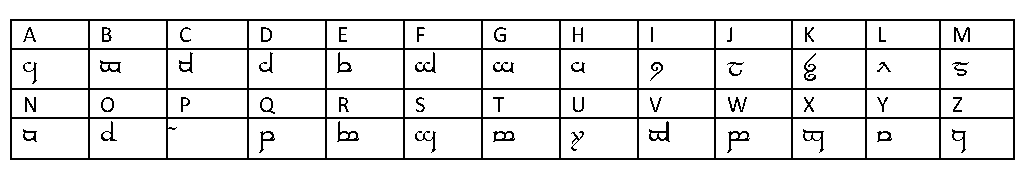
\includegraphics[width=1\textwidth]{../Evne-Ordbog/setup/Alfabeter/Elvisk alfabet.pdf}
    \caption{Elvisk alfabet}
\end{figure}

Elverne fødes fra træernes skyggeside eller dybets mørke, når Måne og Sol mødes i foråret. Det er altid en stor begivenhed, når en elver skabes. De synges med langvarige, magiske remser ud af et gammelt træ eller træernes rødder, i de magiske skove omkring Mek, af den grund sætter de stor pris på deres liv og føler sig hævet over Kalishs andre racer.\\
De magiske omstændigheder for deres skabelse medfører, at deres antal er begrænset; og endnu mere efter Dæmonkrigen, hvor de fleste af elverne døde i forsøget på at beskytte de underlegne racer fra dæmonernes hærgen.\\

\textbf{Højelvere}\\
\textit{Højelverne er beskytterne af Azken Kanpe og magi. De kan stadig finde barmhjertighed overfor de underlegne racer. De bruger de livsskabende energier i Kalish til at være til stede, observere og for at hindre fremtidens Dæmonkrige.}\\
\textbf{Evne:} Hvis en Højelver kan kaste magi, tæller de som at have +2 maksimal mana. Hvis en Højelver ikke kan kaste magi tæller de som at have 2 mana, der genvindes hver time.\\

\textbf{Skovelver}\\
\textit{I skovene omkring Azken Kanpe og ud til Meks grænser lever Skovelverne. De mindes altid de faldne fra Dæmonkrigen, og lever efter at skyde først og spørge bagefter, når det handler om at beskytte Mek. Det rygtes, at Skovelverne kan se de hvileløse ånder, og kan bringe dem til hvile i træerne.}\\
\textbf{Evne:} Som skov elver får man +1 NK og Påfør gift.\\
\textbf{Påfør gift:} Du kan påføre gifte som vil give skade på et våben. Våbnet skal have et blad, så som
kniv, sværd eller ligende, og må ikke være et projektil, så som pile eller en kastet kastekniv. Giften vil kun vare på det næste slag eller til våbnet gives til en anden person,
hvor efter giften vil forsvinde.\\
Når et våben bruges på denne måde skal ordene: "Gift kniv x i skade"siges. Her vil x være hvor meget skade du giver med giften. Skulle giften have andre effekter end skade skal disse ikke siges da de ignoreres.\\


\textbf{Sortelver}\\
\textit{I det dybeste mørke under Livets Ende lever Sortelverne. Deres kvinder har altid det sidste ord. I mellemtiden står alle mændene til på et tidspunkt at tjene i de uendelige kampe mod dværgene. Efter deres gud Daikia døde under gudekrigene har hendes Datter Ishtar taget magten. Alle Daikia's børn er kendt som Ilsherne. Sortelver samfundet er delt op i Huse, repræsenteret med en farve. Ishtars hus er det hvide hus. Sortelvere er sky, arrogante og værdsætter smerte og død.}\\
\textbf{Evne:} Du får evnen Påfør gift og Rygte Spreder/Samler Niv. 1\\
\textbf{Påfør gift:} Du kan påføre gifte som vil give skade på et våben. Våbnet skal have et blad, så som
kniv, sværd eller ligende, og må ikke være et projektil, så som pile eller en kastet kastekniv. Giften vil kun vare på det næste slag eller til våbnet gives til en anden person,
hvor efter giften vil forsvinde.\\
Når et våben bruges på denne måde skal ordene: "Gift kniv x i skade"siges. Her vil x være hvor meget skade du giver med giften. Skulle giften have andre effekter end skade skal disse ikke siges da de ignoreres.\\
\textbf{Rygte Spreder/Samler Niv. 1}
Du kan stille et spørgsmål til en arrangør om, hvad der sker i Akastin eller starte et rygte blandt spillerne.\\
\textbf{Krav:} Som sortelver skal du males sort på alle synlige steder.\\


\section{Grønhuder}
Grønhuderne findes i næsten hele Kalish, men er mest udbredt i de uendelig sletter. Orker er en gåde for de fleste mennesker. Det ene øjeblik kan de virke som harmløse væsner, og det næste kan de gå amok og vil tæske dig med dine egne arme.\\
Ingen ved med sikkerhed hvordan orkerne blev til, eller hvordan de fødes. Nogle orker mener, de faldt ned fra himlen, da der var en stor kamp i gang. Nogle akademikere mener at orkerne er en form for svampeorganismer, der er vokset op af dyngerne af restaffald, som grønhudsgrupperne efterlader.\\
En enlig grønhud bliver set som let bytte af de andre racer, og derfor færdes de sjældent alene. Grønhuder lever for én ting, hvilket er kamp og jagt. De søger altid at jage den største trussel inden for deres leveområde. Det er ikke unormalt, at en grønhud “BOSS” bliver skiftet ud.\\
Grønhuderne viser aldrig frygt - det vil sige, ikke med vilje. Deres primitive levemåde gør dem brutale, og man skal tænke sig godt om, inden man lægger sig ud med dem. For dem er jagten ALT!.
\begin{race*}[Gobliner]
\textit{Goblinen er den mindste grønhud. De holder altid sammen, og ved, hvad der skal til for at overleve, for mange hjerner gør dig klog. Derfor er det oftest goblinerne, der tænker for grønhuderne; men det er stadig bossen, som bestemmer.}\\
\\
\textbf{LP:} 2\\ 
\textbf{NK:} 1\\ 
\textbf{Evne:} Lommetyveri Niv. 1\\
\textbf{Krav:} Makshøjde: 170 cm. Som goblin skal du være malet en lys grøn på alle synlige steder.\\
\rule{\textwidth}{0.4pt}\\
\textbf{Lommetyveri Niv. 1:} Med Lommetyveri Niv. 1 kan du lægge din hånd på offerets pung i 15 sekunder, for derefter at stjæle alt (undtagen de sidste 3 mønter) i pungen. Offeret ved ikke, at de er blevet bestjålet.\\
\end{race*}

\begin{race*}[Ork]
\textit{Orken er grim, stærk og snotdum. De lever for at slås, og for at tage livet af alt, der ikke er med i grønhudstammen.}\\
\\
\textbf{LP:} 3\\ 
\textbf{NK:} 4\\ 
\textbf{Evne:} Bære person\\
\textbf{Krav:} Minimumshøjde: 170 cm. Som ork skal du være malet mørk grøn på alle synlige steder.\\
\textbf{Restriktioner:} Orken snakker meget dårligt menneskesprog, og kender sjældent de rigtige ord for ting.\\
\rule{\textwidth}{0.4pt}\\
\textbf{Bære person:} Du kan nu bære andre personer. Dette kræver fysisk kontakt til personen, samt mere NK end denne, såfremt personen modsætter sig. Benyttelse af denne evne synliggøres ved at sige "bær person", når du ønsker en person skal følge med.\\
\end{race*}

\begin{race*}[Blodork - Kræver specialansøgning]
\textit{Blodorken bliver ikke skabt som de andre grønhuder. Denne form for ork nærmer sig grænsen til det monstrøse. De er større og mere brutale end normale orker, og er resultatet af Hrothgars korruption af orkerne under dæmonernes hærgen. De første blodorker blev til under dæmonkrigene i landet A’kastin, da verden flød med dæmoner og orkerne ikke havde andet føde end dæmonsteg, og ikke havde andet vand end blodet fra dem. Dette gjorde, at de efterhånden udviklede sig til større og mere aggressive orker; blodorker. Blodorkerne er fjendtlige og aggressive, og stort set umulige at nedkæmpe ene mand.}\\
\\
\textbf{LP:} 6\\ 
\textbf{NK:} 6\\ 
\textbf{Evne:} Krigsleder\\
\textbf{Krav:} Minimumshøjde: 170 cm. Som blodork skal du være malet mørk/sort grøn på alle synlige steder.\\
\textbf{Restriktioner:} En Blodork kan ikke snakke med andre end grønhuder. De skal bruge en goblin eller en ork til at oversætte for sig. (Dette er blandt andet for inkludere yngre spillere i voksen spil, dette er derfor et blødt krav som kan ignoreres hvis der ikke er nogen gobliner eller orkere omkring dig.).\\
\rule{\textwidth}{0.4pt}\\
\textbf{Krigsleder:} Når en goblin ser en blodork vil goblinens kampgejst blive forøget. Gobliner som kan se en blodork vil få 1 LP og + 1 NK. LP’et er det første der mistes i kamp og kan ikke genvindes før næste slag.\\
\textbf{Vigtigt!} En goblin kan kun få denne effekt af en blodork. Hvis orkhæren har 3 blodorker vil goblinerne i hæren kun modtage 1 ekstra LP og ikke 3.\\
\end{race*}

\begin{race*}[Trold - Kræver specialansøgning]
\textit{Trolden er alle grønhudernes hemmelige våben. Disse kæmper er utrolig dovne og dumme. I kamp vågner de dog, og trolden er en brutal og nådesløs, der knuser alt på sin vej. Ingen døre eller porte kan holde den tilbage, og trolden kan alene kæmpe sig igennem disse.}\\
\\
\textbf{LP:} 10\\ 
\textbf{NK:} 10\\ 
\textbf{Evne:} Udvidet Naturlig Helbredelse\\
\textbf{Krav:} Minimumshøjde: 180 cm. Som Trold skal du være malet mørk grålig grøn på alle synlige steder.\\
\textbf{Restriktioner:} En Trold kan ikke snakke med andet end grønhuder. De skal bruge en goblin eller en ork til at oversætte for sig. (Dette er blandt andet for inkludere yngre spillere i voksen spil).\\
\rule{\textwidth}{0.4pt}\\
\textbf{Udvidet Naturlig Helbredelse:} Din naturlige helbredelse vil blive forbedret, så du nu vil genvinde 1 LP pr. 5 min.\\
\end{race*}
\chapter{Professioner}
\section{Generelt}
Uanset race, er du nødt til at have en profession, som viser din levevej i A’kastin. Hver profession er blevet givet deres eget regelsæt således, at alle deres regler er samlet ét sted. Dette inkludere en liste over generelle evner, hvilket er evner der ikke er afhængig af din karakters profession. Her står ligeledes beskrevet, hvilke våben og rustningstyper de kan bruge, samt specielle regler der kun gælder for den specifikke profession. Her nedenfor ses en liste over, hvilke professioner der er at vælge imellem. \\

\begin{prof*}[Alkymist]
Alkymisten er ikke særlig god i kamp, men kan lave drikke til at helbrede og forgifte. De kan også forstærke dem selv eller deres kammerater med disse drikke. Hvis man går i kamp mod en alkymist alene så skal man passe på, da et enkelt stik fra en erfaren alkymist kan betyde den visse død.\\
Du kan finde mere information på Alkymisten i Alkymist sættet.
\end{prof*}

\begin{prof*}[Barde]
Barden bruger sin tid på at hygge sig. De synger sange, læser i gamle tekster og samler rygter. De er dog ikke særligt gode til at slås, men derfor kan de stadigt være gode i kamp. Deres evne til at inspirere deres allierede er kun overgået af deres evne til at sprede rygter om deres fjender og deres evne til at skrive magiske skriftruller.\\
Du kan finde mere information på Barden i Barde sættet.
\end{prof*}

\begin{prof*}[Handelsmanden]
Penge får verden til at dreje rundt. Handelsmanden ved dette bedre end alle andre. De kan potentielt skaffe alle resourcer i hele spillet, men dette kræver penge og forbindelser. De er ikke beregnet til kamp, men som den eneste profession som kan købe pistoler så skal man stadig passe på omkring dem.\\
Du kan finde mere information på Handelsmanden i Handelsmands sættet.
\end{prof*}

\begin{prof*}[Helbreder]
Når krigerne falder eller en sygdom spreder sig i landet, så er det helbrederen man har brug for. Ikke nok med at de kan helbreder folk utrolig hurtigt, så er de også i stand til at bruge urter til at helbrede med for at deres patienter kommer hurtigere ind i kampen igen.\\
Du kan finde mere information på Helbrederen i Helbreder sættet.
\end{prof*}

\begin{prof*}[Kriger]
En kriger er den bedste til at slås. Deres evne med et sværd er utrolige. Det er dem som bestemmer hvem der vinder i en kamp. De kan holde til flere slag end den almindelige person, og de kan altid finde arbejde.\\
Du kan finde mere information på krigeren i Kriger sættet.
\end{prof*}

\begin{prof*}[Politiker]
En politiker er ofte midter punktet for en organisation. De har ikke særlig meget magt selv, og vil i stedet finde at deres evner kommer fra de folk der vælger at følge dem. De kan også interagere med verdenen uden for A'kastin nemmere end andre karaktere.\\
Du kan finde mere information på politikeren i Politiker sættet.
\end{prof*}

\begin{prof*}[Skovfoged]
Der er folk som lever i harmoni med naturen. Skovfogeden ved at byen kan være farlig, og ved at udforske skoven så vil de være i stand til at bruge de ressourcer som kan findes mere effektivt. De er også gode til at slås, men ikke helt lige så gode som en Kriger.\\
Du kan finde mere information på skovfoged i Skovfoged sættet.
\end{prof*}

\begin{prof*}[Smed]
En smed er ikke lige så god til at slås som en kriger, men de kan reparere rustning, lave låse, samt forbedre rustning ved at smede runer ind i den, eller fjerne svagheder med Mitril. De er de eneste som kan reparere rustning effektivt og er derfor meget eftertragtede af krigere der bærer tung rustning.\\
Du kan finde mere information på smeden i Smede sættet.
\end{prof*}

\begin{prof*}[Tyv]
En tyv kan stjæle mønter og genstande fra andre spillere. De må ikke tage de sidste tre mønter fra en anden spiller eller genstande så som våben. De kan dog stjæle næsten alt uden at folk opdager det. På trods af at de kun kan bruge bue og kniv, så kan de også snigemyrde selv den stærkeste kriger.\\
Du kan finde mere information på tyven i Tyve sættet.
\end{prof*}
\todo{Indsæt Politikeren}

{\large \textbf{Alle de nedenstående professioner kræver, at der sendes en specialansøgning til arrangørgruppen. Hvordan denne skal skrives og hvad den skal indeholde beskrives i punktet "Karakterskrivning".}}

\begin{prof*}[Druide - Kræver specialansøgning]
Druider kaster magi for at beskytte naturen. Der findes to typer druider. Livsdruider prøver at skabe harmoni, mens Kaosdruider prøver at dræbe alle der skader naturen. En druide kan være utrolig magtfuld, men har sjældent nogen venner til at hjælpe dem.\\
Når du ansøger skal du skrive hvilken type druide du vil ansøge om at spille. Man kan ikke spille begge typer druide, da de fundamentalt strider mod hinanden.\\
Du kan finde mere information på druiden i Druide sættet.
\end{prof*}

\begin{prof*}[Magus - Kræver specialansøgning]
Magus har fået deres magi på usædvanlige måder. Det er sjældent ens fra Magus til Magus. Om det er fra et magisk artefakt eller fordi deres forældre har være magiske væsner. Det betyder også at de ikke er bundet af magi på samme måde, og kan bære rustning lettere, men får ikke nær så mange magier som andre magikastere.\\
Magus er designet til spillere der ikke har brugt magi før. Det er en profession der er relativt overskuelig. Deres fokus er at kaste mange magier fra et lille udvalg.\\
Du kan finde mere information på magusen i Magus sættet.
\end{prof*}

\begin{prof*}[Præst - Kræver specialansøgning]
Præsten hjælper sine krigere i kamp. De er ikke særlig stærke når de er alene. På trods af det er de meget varierede, da hver gud giver deres egen form for magi som kan benyttes. To præster fra forskellige guder kan derfor kaste forskellig magi.\\
For at kunne spille præst, skal du vide hvilken gud du vil tilhøre. Du kan kun skifte religion hvis du får lov til det af en arrangør når du har denne rolle.\\
Du kan finde mere information på præsten i Præste sættet.
\end{prof*}

\begin{prof*}[Shaman - Kræver specialansøgning]
Shamanen er den eneste magikaster som ikke kan kaste magi når de er i kamp. For at gøre op for dette har de mere magtfulde magier. En shaman kan stoppes ved bruge nævekamp eller slå dem med et våben. Man skal dog passe på, da en af de stier som shamanen kan vælge giver dem lov til at bruge skjolde, rustning og våben. Kombineret med deres magier kan de have lige så meget liv som en kriger. Deres magi afhænger blandt andet af hvor mange folk de kan få til at tilbede ånder.\\
Denne profession er god til hvis man er gruppe fra en anden klub. De kræver ikke noget viden om guder, samt bliver stærkere afhængig af hvor mange folk man har med.\\
Du kan finde mere information på shamanen i Shaman sættet.
\end{prof*}

\begin{prof*}[Troldmand - Kræver specialansøgning]
Troldmanden er en varieret magikaster. Nogen er stærke i kamp og kan dræbe folk med en enkelt magi. Andre er snedige og kan få folk til at glemme alt. Uanset hvad, så er en troldmand aldrig særlig holdbar. De har aldrig særlig meget liv og kan som regel dræbes med bue og pil eller en pistol. Der findes flere typer troldmand og du skal vide hvilken type du vil være når du ansøger.\\
\textbf{Dæmonlog} - En dæmonolog bruger deres evner til at kontakte dæmoner. De bruger denne magt til at få deres magier til at vare i meget lang tid.\\
\textbf{Elementalist} - En kamp troldmand. De kan kaste med ildkugler og lave jordskælv. Deres magier er meget effektive i kamp.\\
\textbf{Mentalist} - En troldmand er fokusere på at fordreje sind. Nogen vil mene at de kun er brugbare til at forhøre folk, men de har ikke oplevet hvordan en mentalist kan få deres fjender til at dræbe hinanden.\\
\textbf{Nekromantiker} - Nekromantikeren kan manipulere med sygdomme og livsenergi. De kan lave zombier og spreder døden hvor end de går.\\
Du kan finde mere information på troldmanden i Troldmands sættet.
\end{prof*}

Når man har valgt en profession eller multiclasser til en ny, får man automatisk det første professionsniveau. Ens professionsniveau skrives på ens karakterark som en evne. For at stige i niveau skal man have brugt et bestemt antal XP inden for den profession. Dette XP er det samme uanset profession.
Det antal XP man skal bruge ses i tabellen nedenfor.

\begin{table}[!htbp]
    \centering
    \begin{tabular}{|p{0.35\textwidth}|p{0.35\textwidth}|}
    \rowcolor{cerulean!80}\hline
        Professionens niveau & Krav \\\hline

        Niveau 1 & Ingen \\\hline
        Niveau 2 & 4 XP brugt \\\hline
        Niveau 3 & 8 XP brugt \\\hline
        Niveau 4 & 16 XP brugt \\\hline
    \end{tabular}
\end{table}

Det er muligt at have mere end én profession, hvilket kaldes multiclassing, men dette kræver, at der laves en ansøgning, der skal sendes til arrangørene, og at den profession du gerne vil have adgang til, er relevant for din karakter.
Ved multiclassing vil du blive instrueret i, hvordan du skal forholde dig til modstridende evner og beskrivelser.


\section{XP}
XP er en værdi, der viser, hvor erfaren din karakter er, og hvor lang tid den har været med i spillet. Du modtager 2 start-XP, når du laver en ny karakter, og vil efter hver spilgang, hvor du har deltaget, modtage 1 XP.\\ 
Du bruger XP til at købe evner til din karakter, hvilket kan gøres imellem spilgange, altså off-game.

\subsection{At få nye evner}
Når du køber evner skal du ikke lære dem. Du får dem i stedet givet. Vi vil dog meget gerne opfordre til at man rollespiller at man lærer dem.\\
\textit{Eksempel: Hilda har købt evnen Eksta LP Niv. 1, og hun har dermed 1 ekstra LP på sin karakter. For at give noget sjovt rollespil vælger hun derfor at lære den af byvagts kaptajnen Lucia, hvilket tager form af at Hilda skal beskytte sig mod slag fra slag fra byvagts kaptajnen.}\\

\section{Generelt om evner}
Nogle evner er specielle, da de kræver, at man har en anden evne for at kunne lære dem. Dette gælder evner der henviser til et specifikt niveau. Man kan f.eks ikke købe “Ekstra LP Niveau 3” uden at have Ekstra LP Niveau 1 og 2 først.\\
Det er ikke muligt at købe den samme evne flere gange.\\
Det betyder, at man ikke kan købe “Ekstra LP Niveau 1” to gange, eksempelvis igennem to forskellige professioner.

\section{Multiclassing}
Det er muligt at have mere end en profession. Hvis du ønsker at have flere, skal du først og fremmest have det antal XP, som det kræver. Dit valg skal også godkendes af arrangørgruppen igennem en specialansøgning.\\
Hvis du er helbreder, og multiclasser til kriger, får du adgang til evner og fordele i krigerstien. Du kan dog ikke længere fortsætte med at købe evner fra helbrederstien, så derfor er det vigtigt, at du er sikker i din sag, når du multiclasser.

\subsection{Begrænsninger på professioner}\todo{delete}
Der er dog stadig begrænsninger på multiclassing. En druide, som multiclasser til en kriger må f.eks. stadig ikke bære rustning af metal, ligeledes vil en troldmand der gør det samme heller ikke kunne kaste magi, når de bærer en rustning en troldmand ikke ville kunne bære normalt. En tyv der bære pladerustning, fordi han er multiclasset præst og har taget tempelkriger, vil ikke kunne stjæle, ovs.\\
Denne regel kan forkortes til følgende:\\
\textbf{Du kan ikke bruge evner fra en profession, hvis du bære noget den profession ikke kan bruge.}\\

\subsection{XP Pris}\todo{delete?}
Det koster altid 2 XP at multiclasse, uanset hvad du multiclasser fra og til. Når du har multiclasset starter du på 0 XP i din nye profession. Tidligere brugt XP sættes også til 0.\\
\textit{F.eks. Torben er niveau 3 kriger og vil gerne multiclasse til Shaman. Han har opsparet 3 XP og har brugt 15 XP. Herefter sender han en ansøgning om både at blive Shaman og om at multiclasse til Shaman. Han bliver godkendt til dem begge, han har derfor nu 0 XP opsparet og 0 XP brugt. Han starter derfor i niveau 1 og har kun adgang til niveau 1 som Shaman. Tidligere købte evner tæller altså ikke med i mængden af XP han har brugt som Shaman.}

\chapter*{Efterskrift}
\addcontentsline{toc}{chapter}{Efterskrift}
Når du har læst dette hæfte grundigt, er du klar til at lave din karakter. Har du yderligere spørgsmål eller lignende, så svarer arrangørgruppen gerne.\\
Der kan skrives til vores email: akastin@gmail.com
og til vores \href{https://www.facebook.com/groups/105480345934/?fref=nf}{facebookside} og \href{https://discord.gg/3Ykbtag}{Discord}. 
Til forældre har vi et afsnit på hjemmesiden: \url{http://www.akastin.dk/til-foraeldre}\\
Hvis du, som spiller, har en sygdom eller tager en speciel form for medicin, anser arrangørgruppen det som en nødvendighed, at du eller dine forældre gør os opmærksomme på dette, enten pr. email eller til spilgangen.\\
I forbindelse med sygdomme er det en god idé at have kontaktoplysninger med på en voksen eller forældre, som vi kan kontakte, hvis der opstår problemer. 

\end{document}